\documentclass[11pt,letterpaper]{article}
\usepackage[T1]{fontenc}
\usepackage[utf8]{inputenc}
\usepackage{lmodern,microtype}
\usepackage[margin=0.88in]{geometry}
\usepackage{amsmath,amssymb,booktabs,longtable,array,graphicx}
\usepackage{xcolor,hyperref,fancyhdr,enumitem,xurl}
\definecolor{deep}{HTML}{382064}
\definecolor{accent}{HTML}{7846BD}
\definecolor{light}{HTML}{F4F0FA}
\hypersetup{colorlinks=true,linkcolor=deep,urlcolor=accent,citecolor=deep}
\setlength{\parindent}{0pt}
\setlength{\parskip}{6pt}
\setlist{itemsep=2pt,topsep=4pt}
\pagestyle{fancy}
\fancyhf{}
\fancyhead[L]{\small\textcolor{deep}{AGI ALPHA FLYWHEEL}}
\fancyhead[R]{\small The Capability Advantage}
\fancyfoot[L]{\small Research edition \textbar\ 26 October 2026}
\fancyfoot[R]{\thepage}
\setlength{\headheight}{14pt}
\newcommand{\money}[1]{\text{\$}#1}
\newcommand{\code}[1]{\texttt{\detokenize{#1}}}
\begin{document}
\hypersetup{pageanchor=false}
\begin{titlepage}
\vspace*{0.45in}
{\large\bfseries\color{accent} AGI ALPHA FLYWHEEL\par}
\vspace{0.35in}
{\Huge\bfseries\color{deep} The Capability\\[7pt] Advantage\par}
\vspace{0.28in}
{\Large Game-Theoretic Economics of Skills\\Earned Through Demanding Work\par}
\vspace{0.4in}
{\large SUCCESSOR $\Omega$ Harness\\ACTIVATE. EVOLVE. SCALE.\par}
{\normalsize Powered by Transformational Intelligence $\infty$\\and the applicable AGIALPHA utility.\par}
\vspace{0.5in}
\colorbox{light}{\parbox{0.93\textwidth}{\vspace{8pt}
\textbf{Research question.} Can demanding productive work leave a network with executable capabilities that improve another agent's fresh work, earn their complete upkeep, and finance a worthwhile next investment?
\vspace{8pt}}}
\vfill
\textbf{AGI ALPHA research contribution}\\
MONTREAL.AI project context \textbar\ AI-assisted, same-session independent authoring and review\\
26 October 2026\\[8pt]
\textbf{Evidence boundary.} Executed local scientific-software research; synthetic engineering inputs; authenticated live ENS agents and installed operational adoption not run. Market demand, prices, receipts and financial results are simulations. Actual customer collections are zero.
\end{titlepage}
\hypersetup{pageanchor=true}

\section*{Abstract}

Demanding work can leave a useful executable asset, but a useful asset is not automatically a scarce or financeable advantage. We implemented and tested a connected scientific-software service: solve sparse grounded networks, recover grouped coefficients from partial observations, and optimize a finite-scenario resource allocation. A source-frozen comparison covered 12 engineering chains, three stages per chain and four methods. All 144 arm-stage evaluations passed independent numerical acceptance. An independent agent's reduced-space design method improved the original recipient's solver time by 9.87 and 129.91 times on two separate fresh cases; the reverse acquisition produced no benefit. Competent independent reconstruction was successful and fastest across the complete primary cohort. A searchable registry and a validated skills graph delivered the same accepted work; no incremental graph advantage was demonstrated. A separately frozen finite-cash market model evaluates complete-category cost scenarios, copying, contribution and reinvestment. Demand and monetary inputs remain assumptions, actual customer receipts are zero, and actual all-in research costs are unknown. The evidence supports selective software retention and a recipient-specific execution improvement. It does not establish a durable scarce-capability advantage or realized self-financing growth.

\section{What the work produced}

The delivered asset is an executable scientific workflow, not a transcript: a sparse forward solver, a bounded inverse-calibration method with independently checked predictions, and a robust design method with a numerical optimality certificate. The final design consumes the receiving method's own accepted inverse parameters. Hidden true coefficients never replace a failed upstream result.

The most useful contribution arose during independent construction. Agent A found that repeatedly factorizing the full network inside design optimization was avoidable. Its implementation reduced the design update to the selected edge subspace, using a Woodbury update, analytic sensitivities and constrained optimization. Root retained this contribution as design version 2 before generating primary evaluation inputs. Design version 1 remains preserved as superseded evidence. These are implementations of public mathematical methods; no new theorem or exclusive algorithm is claimed.

\subsection{A visible transfer, including the unsuccessful direction}

The acquisition panel was declared separately and used two new chains with 625 and 2,500 nodes. All twelve stage-method outcomes passed the same independent verifier. The table reports the design solver call only; process startup, native packaging, acquisition and independent verification are excluded from these timings.

\begin{center}
\begin{tabular}{lrrr}
\toprule
Fresh case & Original recipient & Contributed method & Time ratio\\
 & seconds & seconds & original/contributed\\
\midrule
625 nodes & 0.164216 & 0.016639 & 9.87\\
2,500 nodes & 29.279230 & 0.225381 & 129.91\\
\bottomrule
\end{tabular}
\end{center}

\begin{figure}[htbp]
\centering
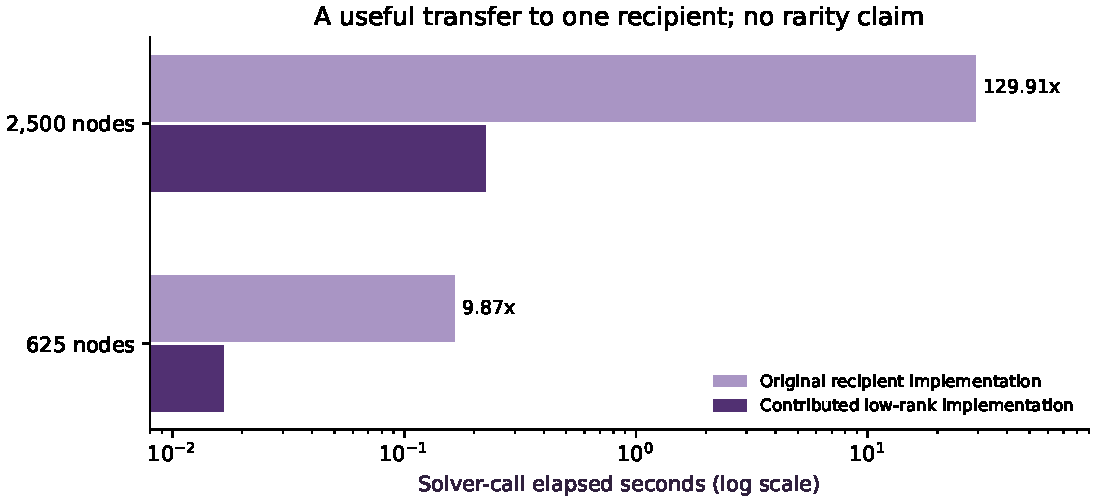
\includegraphics[width=0.94\linewidth]{figures/transfer.pdf}
\caption{An observed implementation advantage for the original recipient. Both methods satisfy the declared numerical contract. This two-case, solver-only comparison does not identify complete monetary acquisition value or a general speedup distribution.}
\end{figure}

The receiving independent agent already possessed the faster method. Importing root's initial capabilities added no accepted task and did not improve its timing. Root's acquisition of the independent contribution is therefore the useful direction. It improves a specific recipient's retained implementation; it does not prove that the independent comparator population lacked the underlying capability. Root's reverse-direction integration time and actual model bills were not separately measured, so a complete observed monetary break-even cannot be computed.

\subsection{Fresh production comparison}

The primary protocol froze all methods and acceptance before input generation. Three fixed seeds at each of four sizes produced 12 independent chains. The four arms were evaluated in a cyclic order, and all 48 inverse outcomes were sealed before downstream design templates were released. No primary repair, favorable substitution or efficacy rerun was used.

\begin{center}
\small
\begin{tabular}{p{0.41\linewidth}rrrr}
\toprule
Arm & Accepted & Complete & CPU & Elapsed\\
 & stages & chains & seconds & seconds\\
\midrule
A: independent retained reconstruction & 36/36 & 12/12 & 99.785 & 98.682\\
B: validated searchable registry & 36/36 & 12/12 & 112.469 & 110.853\\
C: validated skills graph & 36/36 & 12/12 & 114.748 & 113.070\\
D: strong conventional implementation & 36/36 & 12/12 & 182.854 & 181.729\\
\bottomrule
\end{tabular}
\end{center}

These totals include discovery or selection within the invocation, execution, independent numerical checking and the native record boundary. They exclude one-time research construction and catalogue admission, which are recorded separately. All planned rows executed, all complete acceptance budgets were respected, and no additional accepted job was attributable to sharing or graph structure. The 144 evaluations are repeated comparisons of 36 stages in \emph{12 chains}; they are not 144 independent customers or agents.

\begin{figure}[htbp]
\centering
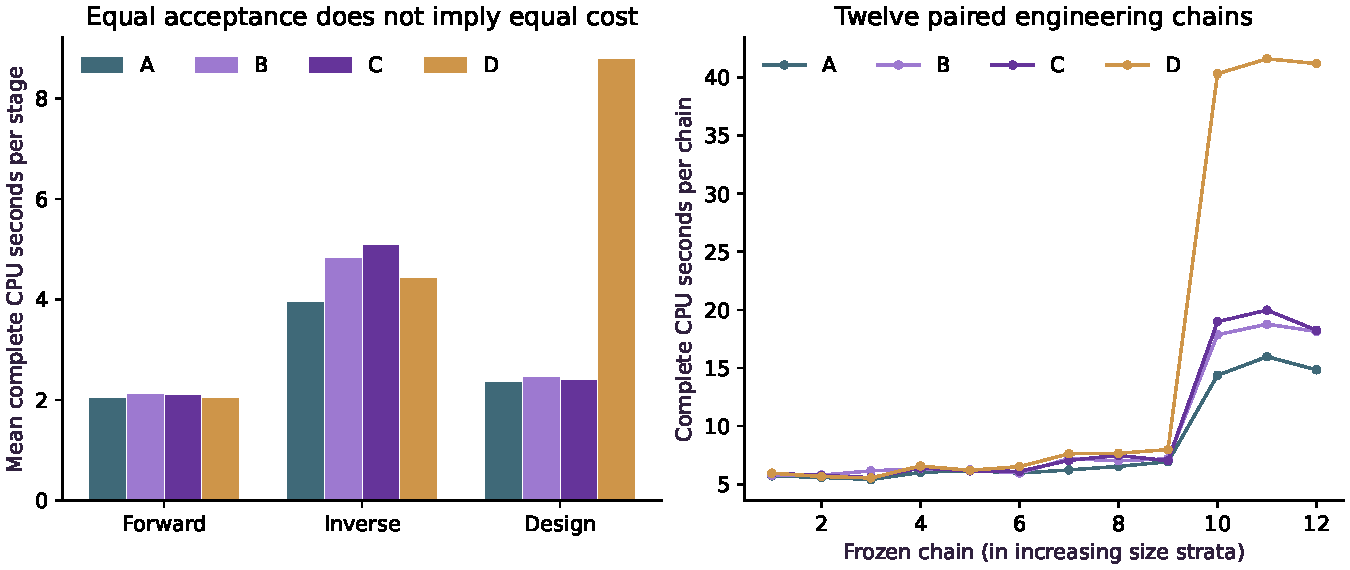
\includegraphics[width=\linewidth]{figures/primary.pdf}
\caption{Complete invocation costs in the frozen primary cohort. Registry and graph use exactly the same selected executable capabilities and evidence. Independent reconstruction remains a strong feasible alternative, including on the largest jobs.}
\end{figure}

The mean paired chain CPU difference was $+1.057$ seconds for B minus A, with a descriptive 95\% chain-bootstrap interval of $[0.403,1.817]$. For C minus B it was $+0.190$ seconds, interval $[-0.066,0.489]$. Positive values consume more CPU. B minus D was $-5.865$ seconds, interval $[-11.569,-0.352]$, primarily reflecting the more efficient design implementation. The intervals resample these twelve chains; they are not population-wide causal estimates, field reliability bounds or evidence about a distribution of foundation models.

\subsection{Success levels and their evidence boundaries}

\begin{center}
\small
\begin{tabular}{p{0.10\linewidth}p{0.25\linewidth}p{0.55\linewidth}}
\toprule
Level & Finding & Supported interpretation\\
\midrule
1 & Demonstrated in scope & Reusable executable numerical capabilities satisfy fresh synthetic engineering requirements. Actual customer demand is unobserved.\\[4pt]
2 & Qualified execution benefit & A contributed implementation improves another recipient's fresh solver performance. No additional feasible job, unsupported baseline capability or complete monetary acquisition benefit is established.\\[4pt]
3 & Not established empirically & Actual complete costs and recurring demand are unidentified. Conditional full-category scenarios are reported separately below.\\[4pt]
4 & Not demonstrated & Graph and competent registry have equal acceptance; graph CPU advantage is not shown, and extra graph authoring cost is unknown.\\[4pt]
5 & Not demonstrated & Actual customer collections are zero; no later-investment bundle qualifies in either sharing arm's 2,304 modeled worlds.\\[4pt]
6 & Not demonstrated & No difficulty-adjusted sequence of independently measured development and validation efficiencies was executed.\\
\bottomrule
\end{tabular}
\end{center}

The result is deliberately narrower than the requested commercial demonstration sentence. This recipient already could complete the work; it completed fresh design work faster after acquisition. The study cannot truthfully replace that finding with ``could not economically perform'' when actual acquisition costs, demand and best-alternative commercial prices are unknown.

\section{Financial results: useful instances, no financed succession}

The market campaign completed all 144 condition/cost cells and 2,304 paired worlds, producing 9,216 primary enterprise histories and 46 additional same-world financing controls. It took 61.995 elapsed seconds and 68.413 process CPU seconds. Process CPU and elapsed time are distinct resource measures; neither measures active authoring effort or human attention. No partial run, seed substitution or outcome-dependent pricing change was required.

The financial result is negative for the proposed accumulating flywheel under the registered test. \textbf{No later-investment bundle qualifies in B or C.} The model does find some worthwhile first assets, but these do not establish a profitable network or fund a repaid sequence of complementary investments.

\subsection{Complete project value versus practical alternatives}

The table counts signs of paired \emph{project-inclusive} value, including completed research prototypes whether adopted or financed by the modeled enterprise. It retains the declared historical allocation. Each cell mean averages its sixteen fixed seeds. Neither the cells nor the worlds are weighted to represent real market prevalence.

\begin{center}
\small
\begin{tabular}{p{0.32\linewidth}rrr rrr}
\toprule
 & \multicolumn{3}{c}{144 cell means} & \multicolumn{3}{c}{2,304 paired worlds}\\
Comparison & Negative & Tied & Positive & Negative & Tied & Positive\\
\midrule
Registry minus independent & 136 & 0 & 8 & 2,217 & 0 & 87\\
Graph minus registry & 0 & 144 & 0 & 0 & 2,304 & 0\\
Registry minus conventional & 113 & 0 & 31 & 1,930 & 0 & 374\\
Graph minus conventional & 113 & 0 & 31 & 1,930 & 0 & 374\\
\bottomrule
\end{tabular}
\end{center}

For registry minus independent, all 768 low-cost worlds have negative project-inclusive value; the reference schedule has 42 positive and 726 negative worlds, and the high-cost schedule has 45 positive and 723 negative worlds. Seven of the eight favorable cell means are merely smaller losses; three favorable cells have zero useful transfers. Only structural condition 20 with reference costs combines a positive B-minus-A mean with a positive B full-project mean: \$5,010.13 versus \$4,968.07 for A. It is reported with all other cells, not substituted for the preselected demonstration. A higher construction-cost scenario can make selected reuse more valuable, but it also increases asset risk. These observations do not justify extrapolating the favorable cells to a market forecast.

The corresponding enterprise ledger comparison, which excludes prototype costs paid outside the modeled enterprise, gives 38 positive, 1,835 tied and 431 negative B-minus-A worlds. Reporting only that ledger would hide part of the project's cost. Prospective deployment, enterprise cash and complete modeled historical/project returns are all retained separately.

Graph and registry make the same cent-denominated financial decisions and have tied project value in every world. With computation left unrounded, C minus B is positive in 49 worlds, negative in five and exactly tied in 2,250. Its full range is approximately $-\$0.0000466$ to $+\$0.0006631$ per world under the declared compute tariff. This is not an exact computational null. It is no evidence of an economically material graph advantage, especially because separate graph authoring cost is unknown and equal fixed allocation is an explicit assumption.

\subsection{Reuse must pay for unused and unsuccessful assets}

Each sharing arm contains 492 modeled asset-construction records across the complete sensitivity panel: 469 G1 records and 23 G2 records, with no G3 adoption. Seventy-three constructions fail, retaining \$5,803.70 of modeled costs per sharing arm across those histories. These sums aggregate distinct hypothetical enterprises and must not be described as actual expenditure or one firm's result.

Only 54 constructed assets receive any use; 438 receive none and retain \$38,577.91 of construction and upkeep costs per sharing arm. There are 840 shared attempts per arm: 835 using G1 and five using G2. One stale use is rejected and costs \$2.00. Acquisition-failure risk is varied and anticipated by buyer/provider choices, but no realized acquisition failure occurs in the selected shared routes. The study does not invent one to populate a requested category.

Thirty-nine G1 asset records have positive terminal direct payback. Their first chronological break-even occurs after two to four attempts, median two. No G2 record repays its direct costs. Its direct net values range from approximately $-\$352.31$ to $-\$3.05$. Thus a useful first asset is possible in the model while the second-stage investment fails to earn its upkeep.

Across the 54 used sharing assets, fully asset-allocated net value per attempted reuse ranges from $-\$55.57$ to $+\$208.30$, with median \$15.36; fifteen are negative and thirty-nine positive. The recipient allocation table contains 493 recipient/asset records, with allocated net value ranging from $-\$55.57$ to $+\$208.30$, median \$28.58. Construction and upkeep are allocated once by each recipient's share of that asset's attempts. The costs of the 438 zero-use assets remain separately charged at network/project level; they cannot disappear because no recipient can be assigned to them. These conditional per-use distributions therefore do not establish positive network value.

Modeled active maintenance spans zero to 26 weeks, with median eight across constructed sharing records; failed constructions have zero active weeks. Useful-life settings of eight and 26 weeks are assumptions, not measured software durability. Observed actual break-even and useful commercial lifetime remain unidentified.

\subsection{Buyers, competitors and contributor incentives}

The behavior model allows abstention, independent construction and conventional purchase. Across the B histories, buyers choose independent construction or use of their retained solution 397,946 times, conventional purchase 130,323 times, the enterprise 114,846 times, and abstention 108,319 times. These are simulated choices, not customers or 397,946 separate constructions. Cheap reconstruction and a good retained baseline frequently remove the provider's proposed advantage.

Repeated weekly investment decisions reject B/C proposals 73,091 times for insufficient forecast complete-cost benefit, 85,694 times because the creator's modeled reward falls below its discovery, validation and integration reservation cost, and 17,019 times for insufficient currently permitted resources. These counts apply separately to each sharing arm; a single decision can have several reasons and a hypothetical enterprise can be counted repeatedly. Copying costs and contributor transfers remain in the complete histories; internal rewards create zero consolidated new revenue.

The factor panel varies network size, diversity, task difficulty, overlap, demand intensity, copying delay, cheaper reconstruction, useful life, acquisition risk, staleness and integration friction. The three-generation dependency sequence is held fixed; complementarity is not separately varied. The panel is balanced on margins, not fully factorial. This design challenges the mechanism under diverse conditions but does not identify an independent causal coefficient for every factor or prove robustness to a stronger foundation model that was never executed.

\subsection{Cash, receipts and the next investment}

The \$200 reserve constrains each new investment decision; it is not an inviolable minimum bank balance. Continuing operating expenses can consume reserves. The independently reconciled minimum cash is \$62.98, while every construction decision respects its obligations and required investment reserve. No modeled enterprise becomes insolvent in the retained campaign.

The B/C models each fund 23 later asset records, but no full G2+G3 bundle is financed, repaid and beneficial against the fixed no-later-bundle control. The conjunction matters: seed cash is not earned surplus, an affordable prototype is not a repaid investment, and one successful component cannot repay an unfunded completed prototype by omission.

The preselected illustrative world---structural condition 01, reference costs, seed 12001---remains in the demonstration even though it makes no sale. All arms receive zero customer collections, accept zero jobs and adopt no capability asset. Prospective operating profit excluding the prior historical allocation is $-\$154.00$ in every arm. Complete modeled project return is $-\$611.16$ for A, $-\$615.78$ for B/C and $-\$611.37$ for D. All finish with \$484.48 of modeled cash, including unspent seed, and zero generated resources available for reinvestment. The graph's visible structure does not change that result.

\subsection{Investment decision supported by this evidence}

Retain the tested reduced-space design implementation for recipients it improves. Do not infer a scarce-capability business from its speed ratio. In this cohort, competent reconstruction, small absolute computation costs, selective demand and the costs of unused assets prevent a demonstrated accumulating, financeable advantage. No graph-specific investment is justified by a measured incremental commercial benefit here.

The actual-cost account has zero observed receipts and unknown all-in construction, inference, human attention and maintenance costs. Empirical Levels 3 and 5 remain unidentified. The scenario account supplies useful conditional failure and payback evidence, but it fails the registered later-bundle succession test. Repeated productive work could replenish an advantage in another domain or demand setting; that remains a hypothesis requiring new preregistered work and actual buyer evidence.




\section{The business decision}

A reusable capability is an asset only when it improves a complete useful outcome enough to cover acquisition, adaptation, verification and upkeep, together with its fair share of construction. A larger collection of skill records is not itself a productive advantage. This study therefore follows a demanding engineering deliverable from a forward model through parameter calibration to a constrained design decision, measures actual executable transfer, and asks what financial conclusions those measurements can support.

The proposed buyer is a computational engineering team that needs a reproducible model and a feasible resource allocation across specified load scenarios. The output supports a decision about where to allocate a limited conductance budget, with numerical evidence for the chosen parameters, predictions and design. It replaces a bounded scientific-programming workflow: build the operator, fit the parameters, perform scenario analysis, optimize, and independently check the result. This is a \emph{market hypothesis}. No buyer interview, customer order, paid pilot or willingness-to-pay observation was obtained.

The underlying mathematical methods are public \cite{scipy}. Our commercial test cannot treat knowledge of sparse factorization, nonlinear least squares or constrained optimization as exclusive intellectual property. The credible mechanisms are recipient-specific execution improvement, avoided repeated construction, reliable integration and maintained evidence. Durable scarcity would require additional evidence that these benefits survive competent reconstruction and competitor response.

Two facts constrain the interpretation from the outset. First, both independent constructors developed complete methods within their actual allowed budgets. Second, the recipient with the stronger independently retained method gained no measured benefit by importing the initial shared methods. Sharing is selective: a capability useful to one recipient can be redundant or worse for another.

\section{Starting evidence and preserved ownership}

This is an additive study under Alpha coordination issue 4850 \cite{alpha}. It does not replace the existing runtime, scheduler, cost calculator, identity infrastructure or publication owners. Exact source inventories and coordination excerpts accompany the study. The inspected current references are:

\begin{center}
\small
\begin{tabular}{ll}
\toprule
Repository & Inspected commit\\
\midrule
Alpha & \code{882456afe59d7bf9493ceaefc79f4f05c0cf7c9a}\\
Fleet & \code{45759fb096faf8988f58ae5ea71248d0f35a97c7}\\
Jobs v0 & \code{bc4abbd5c28f3672275b13300e40ea26c820b8ee}\\
Jobs Manager & \code{5d5670df9dbbc79da115e0a44b71989f34df58c1}\\
\bottomrule
\end{tabular}
\end{center}

The previous first-asset diagnostic reported mean modeled prospective profit of \$183.28 and a \$184.97 advantage over ordinary delivery under its favorable \$20, zero-integration, higher-workload assumptions \cite{prior}. Adding its \$361.52 historical research allocation changed mean profit to $-\$178.24$. The conventional builder tied the retained asset. Those figures belong to that earlier cohort and are not results of the present numerical experiment.

The subsequent second-investment study accepted six full-lock metadata questions in all three arms. Its retained workflow was slower than the ordinary alternatives. Across 1,920 paired modeled worlds, 114 funded research attempts per treatment produced zero qualifying second investments. The separately developed validated-graph study likewise found matching accepted metadata decisions and no demonstrated graph advantage. We preserve these findings and their source identities. We do not replace a failed primary with a favorable later condition.

The present study changes the work family. Alpha's inspected local Workbench numerical adapter performs exact polynomial quadrature; the project already also has competent conventional scientific and scheduling workflows. Their existence rules out claiming that the network lacked all numerical or optimization ability. The missing deliverable is the newly specified, integrated sparse inverse-and-design service, not an absence of general mathematical knowledge.

\section{A connected engineering outcome}

\subsection{Forward response}

For a supplied graph with positive edge conductances and nonnegative grounding terms, the model is
\[
K(c) = B\,\mathrm{diag}(c)\,B^\mathsf{T}+\mathrm{diag}(g),
\qquad K(c)u_s=q_s.
\]
Each connected component must have positive grounding. Here $B$ is an oriented incidence matrix and $s$ indexes the finite supplied load scenarios. The forward deliverable contains the complete state vectors. Independent acceptance assembles its own operator, solves the balance equations, and checks relative state error and backward residual.

The retained forward capability encapsulates input checking, sparse operator construction, factorization reuse and batch solution. Its public numerical dependencies remain available to all comparators. It is executable across different graphs and loads; it is not a saved answer or transcript.

\subsection{Inverse calibration}

The next job asks for bounded grouped conductance multipliers from partial state observations. A returned fit must satisfy parameter bounds, reproduce the supplied observations, solve its own balance equations, and predict responses to additional load vectors. Local identifiability is checked independently. Parameter names or a successful optimization flag cannot establish a well-posed inference.

The shared implementation initially used exact implicit sensitivities and bounded nonlinear least squares. Different independent constructors made different implementation choices, including direct sensitivity solves and factorization reuse. This heterogeneity is concrete source-level behavior within current-session agents; it is not a claim that distinct pretrained foundation models were compared.

\subsection{Constrained design}

The design stage uses the \emph{actual accepted fitted parameters} returned by each arm's inverse stage. It chooses nonnegative conductance additions on selected edges:
\[
\min_{x}\ \max_s q_s^\mathsf{T}K(x)^{-1}q_s,
\quad 0\leq x_j\leq \bar x_j,\quad a^\mathsf{T}x\leq b.
\]
The objective is convex for this positive-definite finite model. The independent checker forms supporting hyperplanes to the scenario objectives and solves a linear program to obtain a global lower bound. Acceptance requires a small numerical gap between the feasible returned objective and that bound. It also checks the resulting design against the separately held true calibrated network.

The independent receiving agent constructed a different reusable method: reduce repeated design evaluations to the selected-edge space through a low-rank update of the base factorization. This avoids repeatedly factoring the entire network during optimization. The contributed implementation remains one immutable asset; the shared library references it rather than counting another copy as growth.

\subsection{Actual transfer and the asymmetric result}

Before primary confirmation, a separately registered transfer panel compared the initial shared methods with the independently retained implementation on two new connected chains. Both methods accepted every stage. Importing the initial shared methods gave the already-capable recipient no additional accepted output and no observed solve-time benefit.

The reverse direction was useful. The original shared design took 0.164216 and 29.279230 seconds on the 625- and 2,500-node tasks; the contributed method took 0.016639 and 0.225381 seconds. These are respectively 9.87 and 129.91 times faster \emph{solver calls} on two development-panel observations, not complete service speedups or estimates of a population effect. Imports, file handling, validation and acquisition remain separate costs.

We selected the contributed design as version 2 before primary inputs were generated, retained version 1 and its results, and required independent combined validation. The no-transfer arm already owned that contribution. No comparator was stripped of its stronger method to manufacture a network advantage.

\section{Protocol, comparators and information custody}

The primary design specifies 12 independent connected chains, four topology/size strata with three seeds each, and three staged jobs per chain. The planned count is therefore 36 staged jobs and 144 arm-stage evaluations. The statistical and natural complete-deliverable unit is a chain; 144 repeated method evaluations do not constitute 144 customers or independent cases.

\begin{center}
\begin{tabular}{lrrrr}
\toprule
Stratum & Nodes & Loads & Inverse parameters & Design variables\\
\midrule
Grid &100&4&4&8\\
Anisotropic grid &625&8&12&24\\
Irregular connected &1600&12&20&48\\
Long-range grid &2500&16&32&80\\
\bottomrule
\end{tabular}
\end{center}

Three 49-node development tasks and two 225/400-node discovery chains precede confirmation. The independent constructor additionally used its own disclosed development stresses; these are not primary data. The two-chain reciprocal transfer panel is also a separate development cohort. All source versions, attempts, failures and protocol amendments are retained.

The independent acceptance owner committed the primary seeds before source freeze. The complete source, policy, evidence, runtime configuration and accepted validation receipt are then frozen. Primary forward and inverse inputs are generated only afterward. Design templates remain unreleased until all 48 inverse arm outcomes, including failures, are sealed. Each design input records its template, parent task, actual fitted result and acceptance hashes. A failed inverse blocks downstream design; the true hidden parameters never replace a failed recipient result.

All source and answer files share the same research filesystem. Role separation and staged disclosure provide process custody, not a cryptographic access-control boundary. The supplied code was checked for hidden-oracle reads; fresh answers do not appear in skill records or retrieval indexes. Reproduction after publication is not a new blind test.

\begin{longtable}{p{0.05\textwidth}p{0.27\textwidth}p{0.60\textwidth}}
\toprule
Arm & Mechanism & Competence retained\\
\midrule
A & Independent accumulated capability & Independently authored sparse forward, exact inverse sensitivity and reduced-space design; ordinary tools, public methods, development tests and reconstruction allowed.\\
B & Validated searchable registry & Current shared capabilities, the same evidence, scoped validation, versioned dependencies and competent indexed search and dependency planning.\\
C & Validated graph & Exactly the same assets and evidence as B; typed graph adjacency for dependency closure and reuse.\\
D & Independent conventional implementation & Separate expert construction with sparse factorization, analytic derivatives and conventional constrained optimization; no forced naive solver or cache removal.\\
\bottomrule
\end{longtable}

All arms receive identical task requirements, numerical acceptance and the existing native 60-second complete-task envelope. A solver subprocess has at most 50 seconds within the remaining allowance. A 70-second outer limit exists only for cleanup and can never turn a late result into acceptance. Matched evaluation order follows a fixed cyclic rotation. No outcome-driven repaired run replaces a primary failure.

\section{What the agents actually possessed}

The constructors used the session-declared GPT-6 Astra Pro model with different task exposure and retained source artifacts. A general integration/testing role independently produced its first complete solver version and validated it across its development panel in a 225.039-second elapsed interval. The foundation/identity role produced the separate conventional implementation in 303.680 seconds. These intervals include communication, checking and waiting. They are not active-human labor measurements or model billing.

Neither constructor needed to acquire the root's source to solve the development jobs. The baseline therefore establishes practical independent reconstruction, not unsupported mathematical capability. A missing skill file at the beginning cannot be counted as failure. Raw pre-construction capability where not directly run remains \emph{NOT RUN}, rather than zero success.

The first recipient's acquisition/integration interval for the initial shared library was 175.825650 seconds, including protocol coordination and harness work. It is not directly comparable with the construction interval as an experimental labor-saving estimate. Root's reverse-direction acquisition time was not separately metered. Thus the measured design execution advantage is real within the tested software, but its complete monetary acquisition benefit remains unidentified.

The six economic success levels are prospective criteria, not a ladder climbed by changing terminology. A working retained executable, a faster recipient, positive complete-cost network value, an incremental graph benefit, financed succession, and improved capability-development efficiency are different claims. The results section reports each at its supported scope.

\section{Validation, identity and execution remain separate}

The foundation papers specify scoped evidence dossiers, controlled admission, versioned executable skills, typed commitments and independently controlled root publication \cite{merkle,proofloops}. Their Merkle inclusion guarantees concern a commitment. They do not establish numerical correctness, useful demand, safe execution or profitable delivery.

This study reuses the preceding graph study's generic authority and commitment implementation unchanged where possible. Its hash profile is explicitly \code{SHA256_RESEARCH_V1}; it is not byte-compatible with the paper's JCS/Keccak profile. GoalOS's inspected reference loop and structural admission do not establish a deployed live validated-skill graph.

The additional validation-attestation policy accepts eligible direct \code{*.agent.agi.eth} identities only within the explicit research fixture. Creator attribution, validation attester, root publisher and local execution permission are separate fields and grants. An ENS-looking name is not authentication. The original Jobs \code{*.club.agi.eth} validator roles, governance and settlement are unchanged.

Admission executes the exact currently declared implementation and independently verifies its fresh numerical outputs. A trusted frozen receipt binds implementation closure, validator, evidence, scope, environment, policy and composition. Cached reuse checks those exact bindings and lifecycle state. This closes the preconfirmation defect in which an old correct answer could have been associated with changed executable code.

Version 2 of the design capability supersedes version 1 for current selection while preserving historical evidence. Revocation, expiry, authority changes, supersession and changed dependencies require refusal or revalidation. A composition is validated as a complete chain, independently of component admissions. B and C use the same acceptance and freshness rules.

The native SUCCESSOR Workbench compiles and records these bounded authored research jobs through its existing adapter interface. It continues to emit \code{PUBLIC_LOCAL_EXECUTION}, admission \code{HOLD}, empty authority and disconnected settlement. Imported packs remain unauthenticated historical evidence. Live ENS authentication, installed Harness/Fleet adoption and customer settlement are \textbf{NOT RUN}.

\section{Economics: whose alternative, whose cost?}

For recipient $i$ and capability $k$, the relevant alternative is the least costly practical accepted outcome available to that recipient:
\[
V_{ik}(n)=
\min\{C^{\rm retained}_{ik}(n),\
C^{\rm reconstruct}_{ik}+C^{\rm rebuilt}_{ik}(n),\
C^{\rm outside}_{ik}(n)\}
-C^{\rm acquire}_{ik}-C^{\rm shared}_{ik}(n).
\]
Failure, adaptation, verification, maintenance and residual attention belong inside these quantities. A successful reconstruction is retained; its construction expense cannot be avoided anew on every reuse. An already-capable agent does not receive an invented capability gain by loading another copy.

At network level, shared construction is charged once. Recipient allocations describe distribution rather than another consolidated expense. Internal contribution rewards are a debit and credit that sum to zero; only external customer receipts create operating revenue. Token issuance and assumed AGIALPHA appreciation contribute zero revenue.

The resource ledger separates measured process CPU and elapsed intervals from unobserved model bills and active human attention. Complete actual cost, historical return and realized profitability remain unknown. The low/reference/high schedules are complete-category scenarios, not invoices, empirical confidence bounds or market prices. They include construction, failed candidates, discovery, validation, integration, execution, retries, verification, upkeep, revalidation and residual attention. Initial root authoring uses an explicitly labeled scenario proxy rather than a fabricated measurement.

The numerical service's complete primary output is a chain. In the market experiment, each purchase is explicitly one separately requested stage service. That distinction prevents the three stages of one engineering deliverable from becoming three claimed real customers. Economic observations are calibrated to the executed stage outcomes and resources, while recurring demand, future reliability, buyer preferences and integration frictions remain model assumptions.

\subsection{Buyers, copying and contribution}

The simulation reuses the existing canonical cost and shadow-ledger primitives and finite-cash helpers. It adds family-specific retained capabilities, acquisition and dependencies. Buyers and agents can choose retained delivery, independent reconstruction, conventional alternatives, shared acquisition or abstention. Offers anticipate declared acquisition and staleness risks. Competitor copying reduces future scarcity and access rents; cheaper reconstruction and high initial overlap directly challenge the sharing mechanism.

The fixed balanced panel varies network size, diversity, task difficulty, recurrence, overlap, copying delay, integration, failed acquisition, useful lifetime, stale capabilities, buyer choice, equal-arm price hypotheses, collection delay and contributor reward. Complementarity is held to the declared three-stage sequence. These are simulated populations, not executed agents. The panel is not a full factorial or a probability distribution over real markets; cell-level results and downside paths must be retained rather than averaging heterogeneous assumptions into a sales forecast.

Contribution occurs only when the modeled expected reward covers the declared discovery, validation and integration reservation cost. Free riding and copying can remove that incentive. The model credits no proof premium, token-price uplift, unmeasured customer review saving or permanent exclusivity.

\subsection{Applicable AGIALPHA utility}

The inspected Jobs integration supports inert transformation intake and a zero-cap AGIALPHA draft; a positive proposal requires its separately authorized charter. The 18-decimal AGIALPHA route remains separate from the Manager's unfunded 6-decimal USDC proposal. Those existing proposal mechanisms are not customer receipts or an authorization to settle this research. This study invokes neither route, assigns no operating income to issuance or appreciation, and does not invent a new token utility to close a financing gap. Live token execution and settlement are not run.

\subsection{Finite cash and succession}

Opening seed funds are distinct from earned resources. Available reinvestment is constrained by both liquid cash after obligations and reserve, and already collected operating-generated resources. A future receivable, customer saving or favorable expected return is not spendable cash.

The model reports prospective deployment value, full historical/project-inclusive return and financeable succession separately. A later-investment bundle must involve the actual tested capabilities, be funded from generated resources, be used on fresh work, repay its complete direct costs including failures, and improve project-inclusive return against the fixed same-seed no-later-investment control. A positive combined control is not evidence that every component separately repaid itself. The research prototypes were constructed before the simulated sales: the exercise is a counterfactual financing test, not a claim that customers funded their historical creation.

\section{Interpretation and operating decisions}

The practical engineering lesson is selective retention. A network should retain a well-evidenced implementation when it improves a recipient's feasible outcome or complete cost; it should decline redundant acquisition, keep strong conventional methods, and retire obsolete versions. The contribution with the clearest observed benefit here is an executable numerical implementation, not a graph record.

The graph and the registry must earn separate verdicts. A competent registry already supports indexed lookup, evidence access and dependency planning. The present graph is small and both mechanisms inspect the same necessary relationships. Any timing difference is descriptive until it exceeds construction, validation and maintenance costs at a relevant workload. Neither cryptographic inclusion nor a growing node count establishes that result.

The study does not establish global uniqueness, autonomous scientific discovery, a deployed ENS-agent economy, paid recurrence, complete research repayment or self-acceleration. The task sequence was planned; the original numerical algorithms were initially prototyped together. Later contribution and supersession are genuine software events, but three stages do not identify a difficulty-adjusted trend in capability-development efficiency.

Useful work need not wait for Level 6. The bounded deliverable can be reviewed as a scientific-software offering, subject to normal software qualification and an explicit operating scope. The next commercial evidence should concern a real recurring need, complete provider/customer costs and a buyer's best alternative. The present finding must not be turned into a claim of an economically scarce network capability merely by attaching a stronger label.

\appendix
\section{Reproduction and evidence inventory}

The companion contains the complete authored implementations, frozen independent baselines, development and transfer evidence, primary tasks and independently held references, per-arm results, native packs, source and protocol freezes, validation/lifecycle controls, market sources, complete scenario histories, cost records and the bilingual demonstration. Reproduction commands and environment versions appear in its README.

The primary solver sources are never silently repaired after their source freeze. Source-formatting diagnostics and unrun repository-wide qualification are reported separately from numerical acceptance. Replaying an archived numerical output verifies that output; rerunning a frozen method verifies executable behavior. Neither is a fresh held-out observation.

The unchanged original Workbench closure, authority/commitment modules and economic primitives retain source identities and licenses. The new integration lives in a separate study namespace. Public release, installed acceptance and any live identity operations remain subject to their existing owners and procedures.

\section{Acceptance thresholds and numerical meaning}

The forward state-relative tolerance is $10^{-7}$ with backward balance error at most $10^{-10}$. Inverse observation fit is checked at $10^{-7}$ and held-out load prediction at $10^{-5}$; local identifiability is checked through a relative singular-value threshold of $10^{-8}$. Design feasibility is checked at $10^{-8}$ and the finite-model global relative gap at $5\times10^{-5}$. The connected design additionally checks true-calibrated-network state error.

These are floating-point numerical certificates for the declared finite model. They are not interval-arithmetic proofs, field measurements, extrapolations to unsupplied scenarios or physical safety approvals. A simulation-generated truth is suitable for this software test but does not provide actual engineering demand or real sensor-model uncertainty.

For completeness, convexity follows along any symmetric affine matrix direction $H$. With $z=K^{-1}q$, the second derivative of $q^\mathsf{T}(K+tH)^{-1}q$ at zero is $2z^\mathsf{T}HK^{-1}Hz\geq0$ while $K+tH$ remains positive definite. Each scenario's tangent plane is therefore a global lower bound; their maximum is a lower bound on the finite-scenario maximum. Minimizing the corresponding epigraph linear program over the original box and resource constraints yields the independent numerical lower bound used here. Floating-point solver tolerances still limit the strength of that certificate.

\section{Cost facts and declared monetary schedules}

The complete primary invocations consume 509.857 process CPU seconds across all four arms. Actual source-bound catalogue admission consumes 6.445 elapsed seconds. Receipt/index construction is attributed 0.456 elapsed seconds from the original root-reported tool duration, not independently remetered. A and D's complete constructor intervals are 225.038953 and 303.680102 seconds, respectively, allocated one third per family. Their included validation, integration and failed-attempt work is not charged again. These elapsed role intervals include coordination and waiting; they are not billed inference or active human hours.

Root authoring was not separately metered. Before primary or market outcomes, its construction-resource proxies were fixed at 300 seconds for forward, 600 for inverse and 300 for original design. The contributed design adds one third of A's constructor interval, giving 375.012984 seconds for the selected shared design record. Shared integration uses an explicitly assumed 200 seconds per family, not the opposite-direction recipient's observed 175.825650-second acquisition interval. Failed shared discovery work retains its measured 2.320419 seconds. All these bases and exclusions appear in the calibration and resource ledger.

The admission and failed-candidate intervals are each divided equally across the three shared families, once within each mutually exclusive B or C enterprise. The original catalogue construction is charged once with G1. The arms are alternative scenarios, so their allocations are not added as actual study expenditure. Admission CPU is not billed again on top of its elapsed-resource charge; each production trial's complete CPU already includes retrieval. The declared 0.1 or 1 reconstruction factor scales construction-resource seconds in all arms, while discovery, validation, integration and the separate catalogue charge retain their own declared bases. Discovery minutes use the research-resource tariff; audit and per-attempt residual attention use the attention tariff. These monetary mappings are assumptions, not additional measurements.

\begin{center}
\small
\begin{tabular}{p{0.48\linewidth}rrr}
\toprule
Scenario assumption & Low & Reference & High\\
\midrule
Research-resource dollars per elapsed hour & 1 & 10 & 100\\
Compute dollars per CPU hour & 1 & 1 & 1\\
Model/tool dollars per build & 1 & 10 & 100\\
Audit minutes per build & 5 & 20 & 60\\
Attention dollars per hour & 30 & 60 & 120\\
Discovery minutes per build & 2 & 10 & 30\\
Maintenance dollars per active asset-week & 0.10 & 0.50 & 2.50\\
Revalidation dollars per event & 0.50 & 2.50 & 10.00\\
Residual attention minutes per attempt & 0.5 & 2 & 5\\
Common setup dollars & 50 & 50 & 50\\
Common weekly dollars & 2 & 2 & 2\\
Preserved historical allocation dollars & 361.52 & 361.52 & 361.52\\
\bottomrule
\end{tabular}
\end{center}

Prices of \$5, \$20 and \$80, buyer value \$50, copying delays, collection delays and other structural conditions are separately fixed in the protocol. The historical \$361.52 is a retained modeling allocation from prior work, not the actual measured total cost of this study. The schedules are assumptions, not invoices or empirically estimated bounds. The actual-cost ledger preserves unknown fields instead of entering zeros. The compressed complete histories contain every modeled bill, invoice, collection, weekly cash snapshot, asset decision, reuse and reserve calculation; the CSVs expose every cell, paired world, asset and recipient allocation.

Validation's rejection behavior and resource cost are tested. Its separate causal effect on commercial reliability or buyer willingness to pay is not identified by an unvalidated-library experiment. Both B and C use the same validation; the model grants neither a proof premium nor an unmeasured human-review saving.

\section{Preconfirmation defects and adverse controls}

Independent review found and corrected source-drift refusal during ongoing development, incomplete elapsed-budget acceptance, missing explicit native-boundary assertions, nonfinite output serialization, timeout process-tree cleanup, archived-answer/current-code admission, self-referential scope matching and repeated catalogue rebuilding. Original outcomes remain in the companion. The invalid-input controls are software tests and count as zero productive jobs.

The economics source review separately required complete-cost symmetry, correct independent-author accounting, buyer anticipation of acquisition risk, failed-transfer costs in repayment, bundle-scoped causal attribution, separation of unknown from unsupported capability, distinct B/C calibration, fractional-cost disclosure and reliable failure finalization. These repairs preceded the registered market outcomes.

\begin{thebibliography}{9}
\bibitem{merkle} MONTREAL.AI project repository. \emph{Merkle Roots for the Validated Skill Graph}, v114. GoalOS commit \code{1e9a5675b1662e98074fb1c71cf2c5b94c7d259f}. \url{https://github.com/MontrealAI/goalos-agialpha-sovereign-machine-economy/blob/main/docs/paper/Merkle_Roots_for_the_Validated_Skill_Graph_v114.pdf}.
\bibitem{proofloops} MONTREAL.AI project repository. \emph{PROOF LOOPS}, v2 author edition. Same pinned GoalOS source. \url{https://github.com/MontrealAI/goalos-agialpha-sovereign-machine-economy/blob/main/docs/paper/PROOF_LOOPS_research_paper_v2_author_edition.pdf}.
\bibitem{scipy} SciPy community. Sparse LU, bounded nonlinear least squares and SLSQP documentation. Accessed 26 October 2026. \url{https://docs.scipy.org/doc/scipy/reference/generated/scipy.sparse.linalg.splu.html}; \url{https://docs.scipy.org/doc/scipy/reference/generated/scipy.optimize.least_squares.html}; \url{https://docs.scipy.org/doc/scipy/reference/optimize.minimize-slsqp.html}. Executed runtime: SciPy 1.17.0.
\bibitem{alpha} MONTREAL.AI. AGI Alpha Agent, Fleet Linux, AGI Jobs v0 and AGI Job Manager source repositories. Exact inspected commits and unchanged native closure in the companion source inventories. Coordination: \url{https://github.com/MontrealAI/AGI-Alpha-Agent-v0/issues/4850}.
\bibitem{prior} MONTREAL.AI. Preserved research contributions: game-theoretic economics, productive transfer, second investment and verified capability. Source/review records: Alpha pull requests 4938, 4939 and 4940 and issue 4850. Their historical results are not pooled with the current cohort.
\end{thebibliography}
\end{document}
